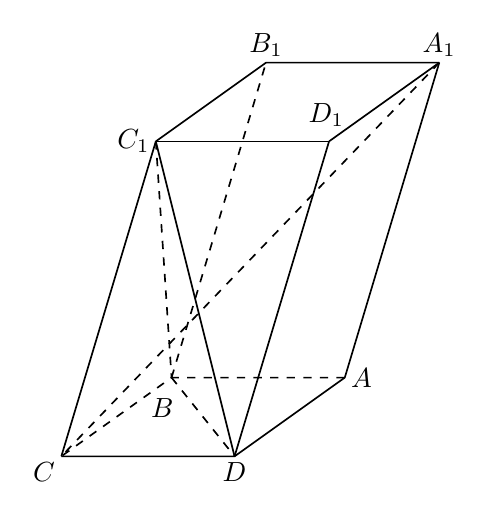
\begin{tikzpicture}[x=1cm,y=1cm,font=\normalsize,line width=.6pt]
\coordinate (C) at (0,0);
\coordinate (D) at (2.2,0);
\coordinate (A) at (3.6,1.0);
\coordinate (B) at (1.4,1.0);
\coordinate (C1) at (1.2,4.0);
\coordinate (D1) at (3.4,4.0);
\coordinate (A1) at (4.8,5.0);
\coordinate (B1) at (2.6,5.0);
% bottom face
\draw (C) -- (D) -- (A);
\draw[dashed] (A) -- (B) -- (C);
% top face
\draw (C1) -- (D1);
\draw (D1) -- (A1);
\draw (A1) -- (B1) -- (C1);
% lateral edges
\draw (C) -- (C1);
\draw (D) -- (D1);
\draw (A) -- (A1);
\draw[dashed] (B) -- (B1);
% triangle C1-B-D on/beside base
\draw (C1) -- (D);
\draw[dashed] (C1) -- (B);
\draw[dashed] (B) -- (D);
% space diagonal A1-C
\draw[dashed] (A1) -- (C);
% labels clear of strokes
\node[inner sep=2pt,anchor=north east] at ([xshift=0pt,yshift=0pt]C) {$C$};
\node[inner sep=2pt,anchor=north] at ([yshift=0pt]D) {$D$};
\node[inner sep=2pt,anchor=west] at ([xshift=0pt]A) {$A$};
\node[inner sep=2pt,anchor=east,xshift=3pt,yshift=-11pt] at ([xshift=0pt,yshift=0pt]B) {$B$};
\node[inner sep=2pt,anchor=east] at ([xshift=0pt]C1) {$C_{1}$};
\node[inner sep=2pt,anchor=south,xshift=-1pt,yshift=3pt] at ([yshift=0pt]D1) {$D_{1}$};
\node[inner sep=2pt,anchor=south] at ([yshift=0pt]A1) {$A_{1}$};
\node[inner sep=2pt,anchor=south] at ([yshift=0pt]B1) {$B_{1}$};
\end{tikzpicture}
